% TODO: write appendices
\appendix
\chapter{Hardware modification enabling serial communication}
\label{appendix:uart_pins}

Here we describe the steps necessary to enable serial communication
between the watch and the PC. On the PC side, serial port will be
emulated through USB, by the same USB debug dongle that is used to
flash program images on the watch. It is a very convenient solution.

We'll start by looking and the USB dongle. Figure
\ref{fig:chronos_dongle_pins} shows the function of the dongle pins.
\begin{figure}[h]
  \centering
  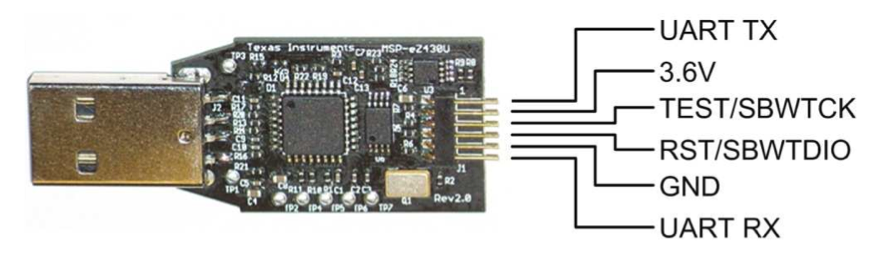
\includegraphics[width=0.7\textwidth]{img/chronos_dongle_pins.png}
  \caption{Pin functions of the USB debug dongle (Courtesy Texas Instruments)}
  \label{fig:chronos_dongle_pins}
\end{figure}
Ones labeled \emph{UART TX} and \emph{UART RX} are responsible for
serial communication. However if you look at chronos watch schematics,
you'll see that these pins remain unconnected in the watch. Relevant
snippet is shown in figure \ref{fig:chronos_unonnected_uart}
\footnote{Schematics are published in \cite{eZ430Chronos} and also
shown in appendix \ref{appendix:watch_schematics} for quick
reference.}.
\begin{figure}[h]
  \centering
  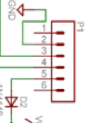
\includegraphics[width=0.15\textwidth]{img/chronos_unonnected_uart.png}
  \caption{Unconnected UART pins on the watch (Courtesy Texas Instruments)}
  \label{fig:chronos_unonnected_uart}
\end{figure}
This is exactly what needs to be changed. Fortunately the MCU is
capable of dynamic port remapping. This means that these UART pins may
be connected to any two IO pins and software can handle rest of the
configuration.

IO pins that are mostly easily connected to the serial lines are those
responsible for watch buttons. The exact location of the connections
is presented in figure \ref{fig:chronos_where_to_connect}.
%TODO(horban): Image goes here
Now we'll describe exact steps necessary to perform the modification:
\begin{itemize}
  \item Take off the  part of the cover that comprises battery compartment.
    Loosen the couplings with a small screwdriver as shown in figure
    \ref{fig:chronos_cover_off}. Ensure you do not lose two tiny
    golden springs that connect power and buzzer to the board.
    %TODO(horban): Image goes here
  \item Prepare two short pieces of wire that will make the
    connections. Take off the isolation. Make sure their length is
    comfortable. Shape them until they form smooth paths between the
    connection points. Ensure that they will not contact to any other
    elements of the watch (SMT resistors near the connector).
  \item Place one of them in position and secure it with tape
    from one side.
  \item Solder the other side to the board. Bonding will now hold the
    wire in position. Remove the tape and solder the other end.
  \item Solder the second wire the same way. End result should
    look similarly to figure \ref{fig:chronos_with_wires}.
    %TODO(horban): Image goes here
  \item Put the cover back on. Ensure that two small golden springs
    are in position.
  \item Test the device, by running TinyOS TestSerial application. See
    it's \emph{README.txt} file for detailed instructions.
\end{itemize}

Note that certain unreliability of the serial port is to be expected.
1 : 1500 error rate is well within tolerance.

%------------------------------------------------------------------------------

\appendix
\chapter{Chronos watch schematics}
\label{appendix:watch_schematics}

\begin{figure}[h]
  \centering
  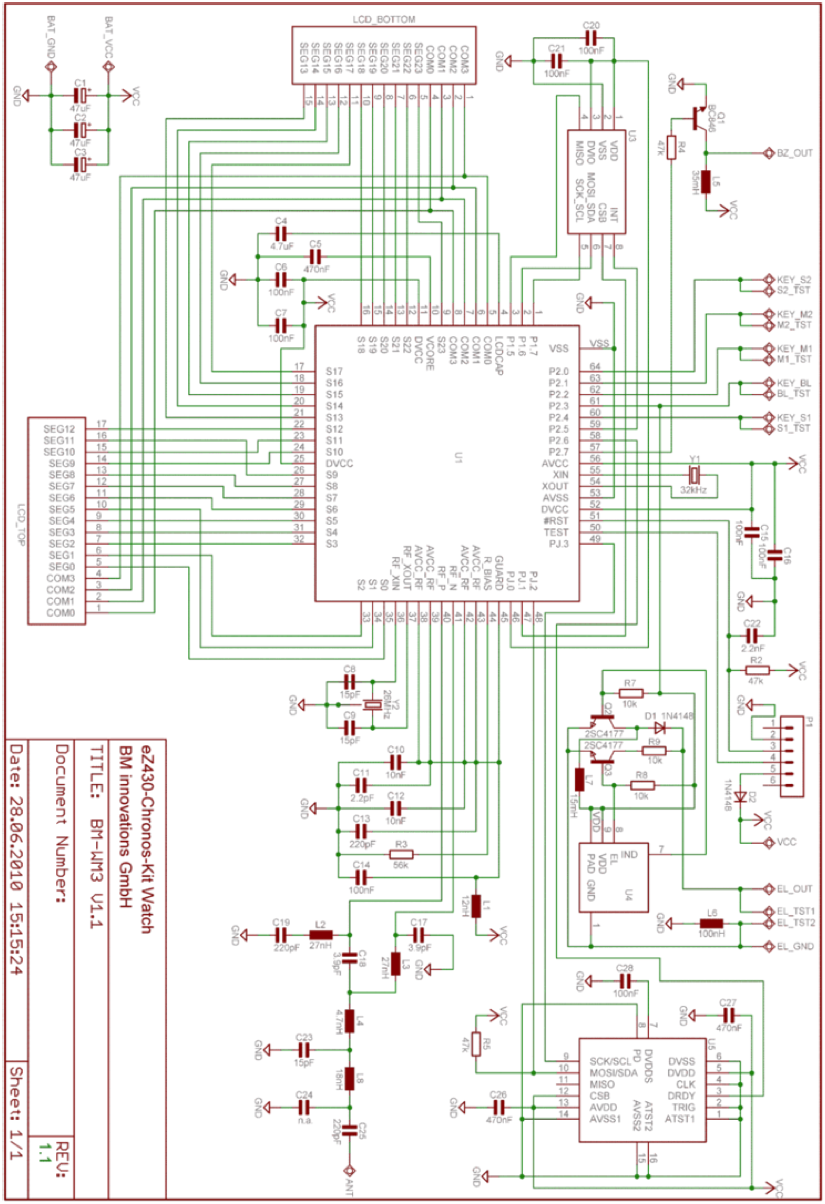
\includegraphics[width=1.0\textwidth]{img/watch_schematics.png}
  \caption{(Courtesy Texas Instruments)}
\end{figure}

\appendix
\chapter{Chronos development environment installation}
\label{appendix:env_install}


% Vim settings:
% vim: set textwidth=70:
% vim: set fo+=t:
